
\section{Guidelines on the approaches used for OpenETCS}


According to  the WP7 decision meeting, the 4th of July, in Paris, SysML, supported by the Papyrus tool,  has been chosen to  cover the highest level of modelling.

The choice of the approaches for the lower levels of modelling is not yet fixed.

This section gives a proposal on how to use the selected approaches to produce from the input documents (ERA documentation and complements)  to a SIL4 code. this section provides also the common structure and convention for modelling, verification and validation activities whatever was the approaches used: definition of the useful data and naming convention.

\subsection{Sum up of chosen approaches and artifacts}

\subsubsection{System analysis}

\paragraph{Aim}
The objectives of this step is to clarify the scope of the study and to provide a detailed description of the chosen solution to cover the requirements of the main input document of the project  [SRS-Subset 26 v3.3.0].

Thus the task of this step  is:
\begin{itemize}
\item to define the scope of the model (more or less the OBU kernel);
\item to provide an architecture for this model (functional and SW);
\item to lift ambiguities;
\item to detect errors and inconsistencies.
\end{itemize}


\paragraph{Input artifacts}

The input documents and elements of this activities are also inputs of the project as this is the first activities.
\begin{itemize}
\item SRS Subset 26 v3.3.0 is the reference document and can be view as a user need document.
\item All the documents provided by ERA according to the directive [CCS TSI ] available \url{http://www.era.europa.eu/Core-Activities/ERTMS/Pages/Set-of-specifications-2.aspx}.
\item Experience of the railway operators partners
\item Experience of the railway manufacturers partners
\item National and Operation Rules of the Operator
\end{itemize}

\paragraph{Output artifacts}

The output shall provide a clear view of the system to design and will be composed of:

\begin{itemize}
\item a set of informal descriptions (scope of the process, description of the functions, behaviour of the system, ...)
\item  an API to  describe the environment of the system to design, its interfaces and its dynamic implementation
\item a functional architecture which identifies the functions to design and the interaction between these functions and with the environment
\item a data dictionary with description of the input and output variables of the system and all the internal variables needed to  describe the system and the interactions between the functions
\item all the requirements, allocated to function or data description, in natural language. The requirements from the SRS can be possibly split and rewritten in order to restrict their scope to the functions or to match the objects of the data dictionary. New requirements can be defined to describe specification choices or to clarify the behaviour of a function (for example according to the experience from a partner). Traceability issue is mandatory and shall be taken into account early.

\end{itemize}

\paragraph{Means}

The first element needed is a way to manage and organize informal descriptions (including text, pictures, tables,...). 

Functional architecture can be easily defined with BDD and IBD diagrams (see \ref{section:sysml}).
Data dictionary  and requirement set shall be tool supported in order to link they contents to the functional architecture and to  be reused during the modelling, verification, validation and safety activities.

As functional architecture, data dictionary and set of requirement shall be linked together, and shall be defined to be used during all the project. Thus section \ref{sec:datamodel} give some specification of the items to defeine and some naming convention.

\subsubsection{Architectural modelling}


\begin{comment}
First decision proposed to use the SysML and Scade approaches for this activity.

Description to provide.
\end{comment}


\subsubsection{Functional and behavioural modelling}


\begin{comment}
First decision proposed to use the SCADE approach for this activity.

Description to provide.
\end{comment}


\subsubsection{Executable software}


\begin{comment}
First decision proposed to use the C language for this activity.

Description to provide.
\end{comment}



\subsection{Data Model}
\label{sec:datamodel}

This section describes all the data shared by the different activities during the project.
These data shall be managed in a common repository which shall be the reference for specification, modelling and VnV activities.

Thanks to the choice of Eclipse platform, use of technologies available on Eclipse and XML files are the best candidates to stores these items.

In the following, we give the specification of these items and the links between them. The specification of this data-model is based on an Ecore model.

3 groups of data are defined: \emph{Variable}, \emph{Function} and \emph{Requirement}; for each group, a set of \emph{attributes} are defined to specify the group. These attributes are specified by a name, a cardinality and a type which can be a well  know type  (as boolean, string, integer,...) or a type defined explicitly for this model.

All these items share common attributes described in the following section. The Features are defined to organize the items in group.
Finally the links between the groups are specified in the last section.


\subsubsection{Common attributes}

All the items are \textit{named} and have mandatory common attributes:
\begin{description}
\item [name] defined as a string and unique, naming convention are defined in \ref{sec:naming};
\item[safety], a boolean tag to qualified the information as safety or not ;
\item[definition], to describe in a clear way the items, at list by a textual description. links to picture or table can be added.
\end{description}

Some \textit{issues} can be associated to  each items. These issues are characterized by:
\begin{description}
\item[description], textual explanation;
\item[closed], a boolean tag to qualified the state of the issue.
\end{description}

\begin{comment}
TODO: do we need more information on issue , as author, owner,... ?

Do we need to link to github issue tracker ?
\end{comment}

The figure \ref{fig:Common} gives the Ecore model of these elements.

\begin{figure}[ht]
  \centering
  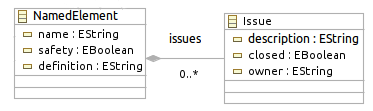
\includegraphics{DataModel/Common2.png}
  \caption{Common attributes for all items}
  \label{fig:Common}
\end{figure}


\subsubsection{Variables}
\label{sec:var}


First of all we have to define the types used to specify the variables.

In order of possible, we shall use simple and well defined, as boolean, string, integer,... (see the Iso standard for C language \url{http://www.open-std.org/jtc1/sc22/wg14/www/docs/n1124.pdf}). 5in the Ecore model these types appeared with the prefix "E").

Besides some new types can be define to define a complex or structured type or an enumeration.

These types are defined as \textit{VariableType} with the following attributes:
\begin{description}
\item[parentType], optional, in the case the type is a subtype of a  already defined type (for example "Distance" can be considered as subtype of "Integer");
\item[minimalValue], optional, in the case the type is a range of integer, the minimal value;
\item[maximalValue], optional, in the case the type is a range of integer, the maximal value;
\item[resolution], optional, in the case the type is a range of integer, resolution to take into account;
\end{description}

The figure \ref{fig:Type} gives the Ecore model of these elements.

\begin{figure}[ht]
  \centering
  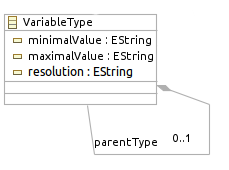
\includegraphics{DataModel/Type3.png}
  \caption{Type definition}
  \label{fig:Type}
\end{figure}

The \textit{Variable} is then defined with the following attributes:
\begin{description}
\item[type], the variableType associated, unique;
\item[definitionRequirements], at least one requirement to  define the variable;
\item[constant], a boolean tag to qualified constants;
\item[specialValue], optional, several special value can be defined;
\item[store], optional, a variable can be an element of a more complex or structure variable.
\end{description}

The figure \ref{fig:variable} gives the Ecore model of these elements.


\begin{figure}[ht]
  \centering
  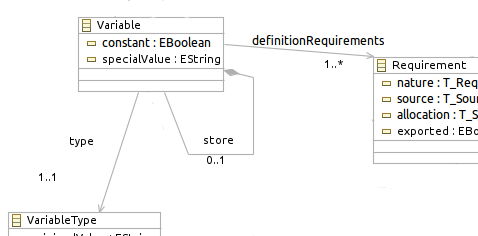
\includegraphics{DataModel/Variable3.png}
  \caption{Variable definition}
  \label{fig:variable}
\end{figure}



\subsubsection{Functions}

A Function is defined with the following characteristics:
\begin{description}
\item[allocation], the subsystem  on which is allocated the function (i.e. Kernel, DMI, Odometry,..);
\item[requirement], at least one requirement to describe the function;
\item[input], optional, the input variables of the function;
\item[output], optional, the output variables of the function;
\item[internal], optional, the internal variables of the function;
\item[subFunction], optional, the sub-functions which allow to structure and  detailled the function.
\end{description}

The figure \ref{fig:function} gives the Ecore model of these elements.

\begin{figure}[ht]
  \centering
  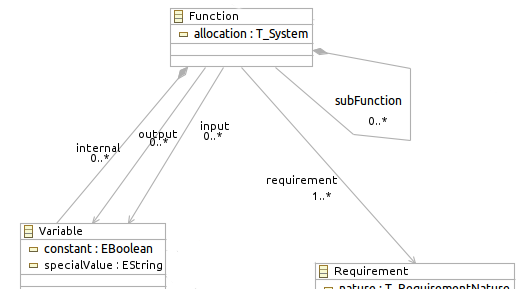
\includegraphics{DataModel/Function1.png}
  \caption{Function definition}
  \label{fig:function}
\end{figure}

\subsubsection{Requirements}
\label{sec:req}

A \textit{requirement} is defined by the following attributes:
\begin{description}
\item[nature], class of property defined by the requirement: Structural, functional, definition,...
\item[source], the document or the artifact where the requirement is defined for the first time (i.e. SRS, SystemAnalysis,...);
\item[allocation], the subsystem  on which is allocated the function (i.e. Kernel, DMI, Odometry,..);
\item[exported], a boolean tag to defined if the requirement shall be exported to another sub-system or function;
\item[subRequirement], optional, the sub-requirements in which the requirements is divided.
\end{description}

Thus the following enumerate sets shall be defined:
\begin{description}

\item[T\_SourceDocument], set of source document for defining a data, this can be an input document (SRS, a subset,...) or a document provided during the process (system analysis, model description,...) 
\item[T\_RequirementNature], what describe the requirement ? Structural, Functional or Definition
\item[T\_System], on what subsystem is allocated the data ? Kernel, DMI, BIU,...
\end{description}

The figure \ref{fig:requirement} gives the Ecore model of these elements.

\begin{figure}[ht]
  \centering
  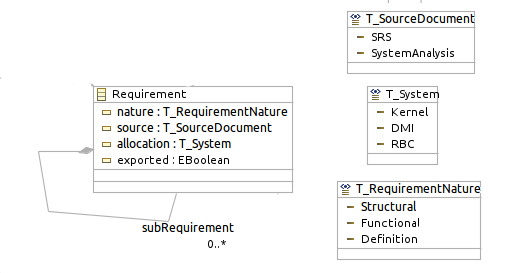
\includegraphics{DataModel/Requirement1.png}
  \caption{Requirement definition}
  \label{fig:requirement}
\end{figure}


\subsubsection{Feature}

A \textit{feature} is a mean to structure the analyse of the system, it is the starting element of an analysis, and contents informal information:
\begin{description}
\item[description] an informal and textual description of the functionality to analyse, which can contain some links to pictures or tables;
\item[subFunctions] the functions which are defined to describe the functionality.
\end{description}

The figure \ref{fig:feature} gives the Ecore model of these elements.

\begin{figure}[ht]
  \centering
  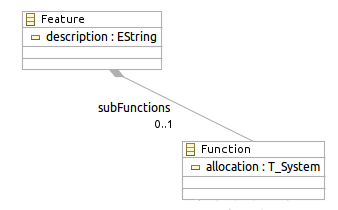
\includegraphics{DataModel/Feature1.png}
  \caption{Feature definition}
  \label{fig:feature}
\end{figure}

\subsubsection{Links}


The figure \ref{fig:links} gives the Ecore model of all the data model as describe above and can be read as an UML diagram.

\begin{figure}[ht]
  \centering
  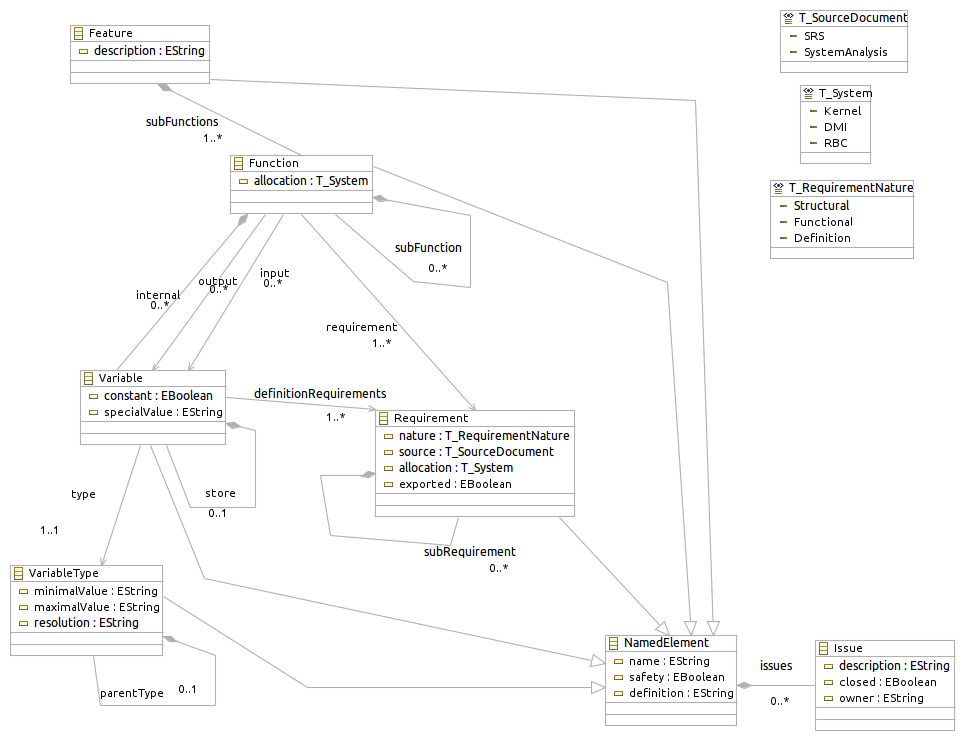
\includegraphics[width=\textwidth]{DataModel/datadictionary.png}
  \caption{General Ecore model of the data dictionnary}
  \label{fig:links}
\end{figure}

\subsection{Name convention}
\label{sec:naming}


\subsubsection{Variable naming convention}

\begin{comment}
How to name object ? base : subset 26 §7.3.2:
" 7.3.2.11 All Variables have one of the following prefixes:
\begin{itemize}
\item A\_ Acceleration
\item D\_ distance
\item G\_ Gradient
\item L\_ length
\item M\_ Miscellaneous
\item N\_ Number
\item NC\_ class number
\item NID\_ identity number
\item Q\_ Qualifier
\item T\_ time/date
\item V\_ Speed
\item X\_ Text
\end{itemize}


\end{comment}


\begin{comment}
Case sensitive language, keywords of target language (SysML, B, C, Scade 5?),...), UPPER case for names issued form official document (SRS, API,...), lower case for others. length of the name

QA plan to check.
\end{comment}


\subsubsection{Function naming convention}


\begin{comment}
TODO: Marc Behrens
\end{comment}

\subsubsection{Requirement naming convention}


\begin{comment}
TODO: Marc Behrens
\end{comment}

